The next prototype, TRITIUM-IFIC 1, was intended to overcome the problems and limitations found in the previous one, TRITIUM-IFIC 0, section \ref{subsec:TritiumIFIC0}. To do so, some improvements were applied on it:

\begin{enumerate}

\item{} The fiber bundle is arranged straight to optimize the photon collection efficiency of the fibers.

\item{} A special fiber cleaning protocol, explained in section \ref{subsec:CleaningProcess}, was applied on the fibers. It was used to improve the interfaces between fiber and tritiated water, creating a better wetting property of the fiber, which will improve the photon collection efficiency of the scintillating fibers.

\item{}  Teflon vessel was using in the Tritium prototypes to reduce the effect of the small photon collection efficiency of the fibers, measured in section \ref{subsubsec:CharacterizationFibers}, which is an innerent characteristic of the fiber which cannot be changed.

Teflon is an interesting material for its optical properties, specifically its reflection factor, which is very close to $100\%$ at the working wavelength. It means that the photons that escape from the fiber will hit the Teflon walls and go back to the scintillating fiber.

\end{enumerate}

The TRITIUM-IFIC 1 prototype consists of 64 scintillating fibers, with a length of $20~\cm$, that are arranged in a straight position using a teflon structure, shown in Figure \ref{fig:TeflonStructureFibersTritiumIFIC1}. The fibers are fixed in an $8\cdot{}8$ square matrix.

\begin{figure}[h]
\centering
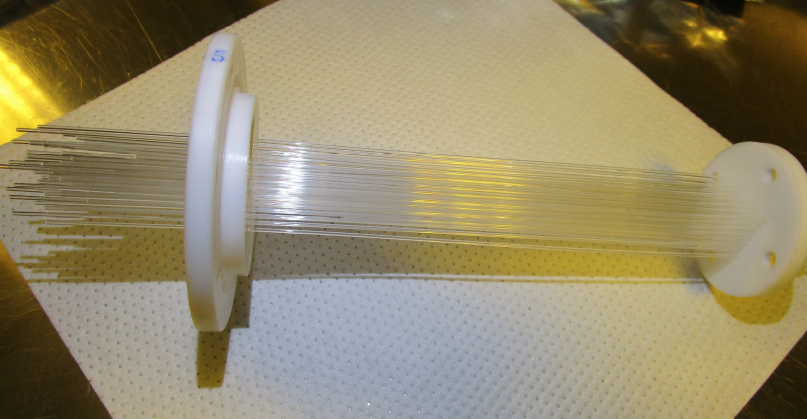
\includegraphics[scale=0.4]{5Prototypes/52PreliminarPrototypes/522TritiumIFIC1/FiberMatrixTeflonStructure.png}
\caption{Teflon structure used to arrange the fibers of TRITIUM-IFIC 1 prototype in a matrix of $8\cdot{}8$.\label{fig:TeflonStructureFibersTritiumIFIC1}}
\end{figure}

A new teflon vessel was designed and built, shown in Figure \ref{fig:TeflonVesselTritumIFIC1}. It has a cylindrical hole whose internal diameter and length are $48~\mm$ and $200~\mm$ respectively, where the fiber structure will be placed. 

\begin{figure}
\centering
    \begin{subfigure}[b]{0.30\textwidth}
    \centering
    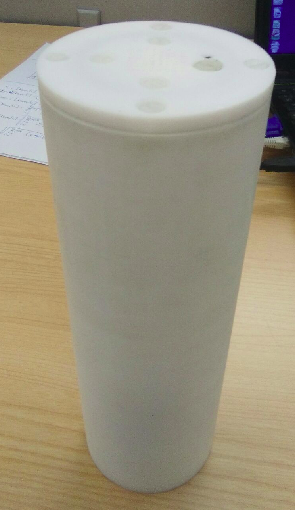
\includegraphics[width=\textwidth]{5Prototypes/52PreliminarPrototypes/522TritiumIFIC1/TeflonVesselTritiumIFIC1a.png}  
    \caption{\label{subfig:TeflonVesselTritumIFIC1a}}
    \end{subfigure}
    \hfill
    \begin{subfigure}[b]{0.45\textwidth}
    \centering
    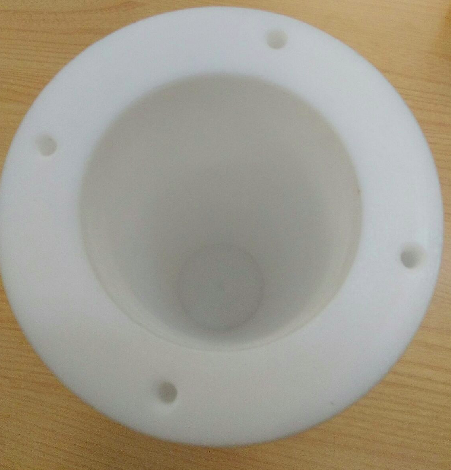
\includegraphics[width=\textwidth]{5Prototypes/52PreliminarPrototypes/522TritiumIFIC1/TeflonVesselTritiumIFIC1b.png}  
    \caption{\label{subfig:TeflonVesselTritumIFIC1b}}
    \end{subfigure}
 \caption{Teflon vessel of TRITIUM-IFIC 1 prototype.}
 \label{fig:TeflonVesselTritumIFIC1}
\end{figure}

In addition to cutting and polishing the scintillating fibers, a cleaning process, described in section \ref{subsec:CleaningProcess}, was applied to them to achieve a better tritiated water-fiber interface.

A piece of PVC was used to fix the photosensor on the prototype and prevent the photosensor from being affected by external light. A general view of this prototype is shown in Figure \ref{fig:TritumIFIC1}, which, for radioactivity safety reasons, will be read using only one PMT.

\begin{figure}
\centering
    \begin{subfigure}[b]{0.40\textwidth}
    \centering
    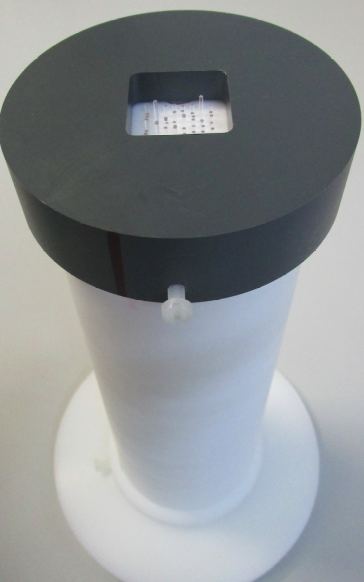
\includegraphics[width=\textwidth]{5Prototypes/52PreliminarPrototypes/522TritiumIFIC1/TritiumIFIC1a.png}  
    \caption{\label{subfig:TritumIFIC1a}}
    \end{subfigure}
    \hfill
    \begin{subfigure}[b]{0.40\textwidth}
    \centering
    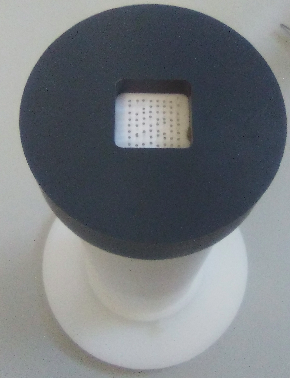
\includegraphics[width=\textwidth]{5Prototypes/52PreliminarPrototypes/522TritiumIFIC1/TritiumIFIC1b.png}  
    \caption{\label{subfig:TritumIFIC1b}}
    \end{subfigure}
 \caption{A general view of TRITIUM-IFIC 1 prototype.}
 \label{fig:TritumIFIC1}
\end{figure}

The PMT used was the model R8520-460, from Hamamatsu Photonics company \cite{DataSheetPMTs} and it was coupled directly to the fiber bundle using optical grease \cite{OpticalGrease}. The electronic circuit, shown in Figure \ref{fig:VoltageDividerCircuit}, was used to distributed the high voltage between the dynodes. The employed high voltage was $-800~\volt$, at which, its quantum efficiency is $28.66\%$.

The signal from this PMT was processed and analyzed using the same electronic configuration as that used for the TRITIUM-IFIC 0 prototype, shown in Figure \ref{subfig:ElectronicConfiguraiton1PMT}.

Unlike the previous prototype, only one TRITIUM-IFIC 1 was built. First, it was filled with ultrapure water ($118~\milli\liter$, uncertainty of $0.05\%$) and several background measurements were taken over a week. Then, it was emptied and refilled with $118~\milli\liter$ (uncertainty of $0.05\%$) of the radioactive liquid source of tritiated water with the same activity as the one used in TRITIUM-IFIC 0 prototype, $99.696~\kilo\becquerel/\liter$.

The results of these measurements are shown in section \ref{subsec:ResultsTritiumIFIC1}, where they are discussed and compared with the result obtained with the previous prototype, TRITIUM-IFIC 0.